\chapter{EXAMINATION OF PREVIOUSLY-EXISTING GLOBAL DP LIBRARIES}

The first goal of this Thesis is to examine previously existing programming libraries and APIs that provide the application of Differential Privacy to a dataset. This has been achieved by many companies, such as Google and IBM, but also from research programs like ARX that study the benefits of data privacy. We separate those implementations regarding their output. The possible outputs of a mechanism that adds D.P. to a dataset can be:
\begin{itemize}
    \item An answer to a query, in a private manner.
    \item An anonymized dataset, that meets the criteria of D.P.
\end{itemize}

In the first category, we can distinguish libraries such as Google's and IBM's, that have functions which if applied on a dataset, and given a specific query, can return a single answer.

In the second one, we can find libraries such as the ARX tool, that given a dataset and a group of privacy settings (such as the amount of noise to be inserted), produces an anonymized version of a dataset, that has obviously reduced information in comparison to the original one, but is usable by the final user.

In this chapter, we are going to test those libraries by providing different kinds of datasets, in order to determine the advantages and the disadvantages of each category.

We are going to conduct all of our testings using noise generated by the \textbf{Laplace Mechanism}, thus we must first define its theoretical behavior.



\section{The Laplace Mechanism}

The Laplace Mechanism is used widely in applications of Differential Privacy regarding \textbf{numerical queries}, which are actually functions that match a query to a number, or a vector of numbers, thus answering to it. The mechanism uses noise produced by the Laplace probabilistic distribution, which is equivalent to the query's sensitivity.

\subsection{Query Sensitivity}
The $l_1$ sensitivity of a query $f$, is defined as following:

\begin{align*}
    \Delta f = \max_{\{||x-y||_1 = 1\}} ||f(x) - f(y)||_1
\end{align*} where $x,y \in N^{|X|}$.

This quantity shows the effect by which a single participant's data can change in the worst case during the query $f$, and thus, the uncertainty that we must insert to to the response in order to protect them.

\subsection{The Laplace Distribution}
The Laplace Distribution with a scale $b$, is the distribution with probability density function: 
\begin{align*}
Lap(x|b) = \frac{1}{2b}exp(-\frac{|x|}{b})
\end{align*}

who's variance is $\sigma^2 = 2b^2$, and is actually a symmetric version of the exponential distribution.

\subsection{Use of Laplace in D.P.}

In order to be of use in our definition, the scale of the noise will be calibrated to the sensitivity of the query $f$, divided by epsilon. Thus, the noise used will be drawn from

\begin{align*}
Lap(\frac{\Delta f}{\epsilon})
\end{align*}

Of course, many other probabilistic distributions can be used to ensure differential privacy, but during our testings we prefer to use Laplace.

\section{Query Answering Libraries}

We are going to begin by testing libraries that belong in the first category, and specifically the \textbf{IBM's diffprivlib}, which is written in python, and is publicly available \href{https://github.com/IBM/differential-privacy-library}{here}. The library includes a host of mechanisms, the building blocks of differential privacy, alongside a number of applications to machine learning and other data analytics tasks. We are going to focus our testings in the simple queries, such as the \textbf{mean value}, the \textbf{extreme values} and the \textbf{histograms} of a numerical dataset. The library consists of three modules:

\begin{itemize}
    \item \textbf{Mechanisms}, as known from the theoretical foundations of D.P.
    \item \textbf{Models}, especially machine learning models, that will not concern us during this thesis
    \item \textbf{Tools} that will allow us to apply D.P. in datasets.
\end{itemize}

We are going to use the tools available, in order to apply differential privacy in a dataset of our own, guided of course by the mechanisms provided by diffprivlib. First, we are going to take a look at the dataset that we are going to use going forward.


\subsection{Setup of the mechanism}

The first step in order to test the library, is to setup the mechanism by defining its properties and parameters. 

\subsubsection{Bounds' Selection}

One of the most important aspects for us if we want to apply DP algorithms, is to define the bounds, i.e. the range that a variable can be in. It would be very convenient in our case to just take the tuple of the smallest and the largest value in the column that we are interested in. However, in the real world, the person who asks the queries is not supposed to know this info about the dataset. Thus, since a solution is not provided by the library, we must define our own bounds by guessing the lowest and the highest values in the fields that we want to examine. 

Thus, the user must have somewhat of a previous knowledge regarding the dataset, in order to decide the minimum and maximum value. Those values do not need to be precise, although the more close they are to real ones, the best the protocol will function. At the same time, we must be sure that during our selection we do not leave some of the dataset's values outside of the bounds, as they will be ignored in the final results. 


\subsubsection{Privacy Budget}

In this form of D.P., someone trying to breach the users' privacy, could theoretically ask an infinite number of questions, and thus each time gain more and more information about their private data. This is not covered by the definition of D.P., however it is not acceptable. In the same manner, an untrusted user of the library could ask the same question many times, aiming to determine how much noise is added each time, in order to find out the actual answer to the query, as the way that the noise is drawn is already known.

In order to eliminate this problem, a special parameter call the \textbf{privacy budget} is implemented. The library offers the ability to initialize this budget before asking any queries. During the queries, this budget is each time decreased, according to how much data the answer to the question reveals. For example, the answer to the "mean value of the charges for a surgery", costs less than the answer to the "histogram values of heart transplant surgeries in the West coast".

This parameter is implemented by the library as the budget accountant. This variable tracks the privacy spent, so that our system is not left exposed after lots of "expensive queries". The system will allow someone to ask one question that uses the whole privacy budget, or a series of questions whose total impact is less or equal to the initial budget.

\subsection{Testings' goal}

When applying D.P. mechanisms to our data, we provide the privacy settings of our choice (epsilon variable), and obtain an answer to each of our questions. Thus, in our testings, our goal is to \textbf{determine the accuracy of the answers}, given a specific ε, or some other settings, and comparing them to the true answer, using some metrics. Those metrics are different for each query type. In this section we are going to focus on two types of queries: statistical, and histograms.

\subsection{General techniques}
In each one of our following testings, we are going to run the query \textbf{many times}. As we already know, D.P. relies on probabilistic algorithms that can some times produce extreme results. This may be rare, but we want our testings and conclusions to be accurate. So, we are going to run each query 100 times, and return as a result the mean value of those runs.

\subsection{Statistical Queries}

The first type of queries that we are going to test are those that answer questions like "What is the mean cost of a surgery?", or "What is the largest fee paid by medicare for a transplant?", known as statistical queries. 

\subsubsection{Metrics used}

In the case of statistical queries, their answer is usually a real number, so in order to check their alteration with the true answer, we are going to take into account the \textbf{absolute difference between the truth and the query answer}. 

\subsubsection{Bounds Definition}

We are considering fees for surgeries in our example, thus a logical lower bound would be 0\$ (surgeries could be done pro bono too!), and an upper bound would be 1 million dollars. Either way, we are trying to be extreme with our picks, in order to not find ourselves in the unfortunate situation that a value taken into consideration by the DP query would be out of bounds.

\subsubsection{The identity of the testing Dataset}

The dataset chosen to test the library, is the publicly available "Surgery Charges Across the U.S.", that contains many different kinds of surgeries in a plethora of different hospitals. Our goal is to protect each hospital's data when it comes down to a specific surgery, while helping a patient choose one, depending on the charges that can be found all over the United States. The data provided in this dataset, is going to help a potential patient balance his need of top care, and the need to spend less money. The columns contained in the dataset are:

\begin{itemize}
    \item Surgery code and definition
    \item Provider hospital name
    \item Provider city
    \item Average total payments
    \item Average medicare payments
\end{itemize}

We are going to focus on the last two columns, in order to approximate the charges of a surgery. The above table gives us an image of the containers of the dataset.

The dataset contains a total of 200,000 entries, a more than satisfying number for running D.P. algorithms.

\begin{table}[!htb]

    \caption{"Surgery Charges Across the U.S." dataset columns}
    \label{numbers}

    \begin{tabular}{| c | c | c | c | c| c |}
      \hline 
      ID & Surgery Type & Hospital Name & Hospital City & Total & Medicare \\
      \hline
      1 & TRANSPLANT & MAYO CLINIC & PHOENIX & \$240422.80 & \$133509.55\\
      \hline
      2 & ECMO &  GROSSMONT HOSP & LA MESA & \$193617.86 & \$192003.43 \\
      \hline
      3 & CRANIOTOMY & STANFORD HOSP &  STANFORD & \$32597.87 & \$29347.12  \\
      \hline
    \end{tabular}

\end{table}

\subsubsection{General Dataset Utilities Queries}

Our first experiment is just to ask for some of the utilities of the dataset, and specifically its cost column: the \textbf{mean value}, the \textbf{variance}, the \textbf{sum} and the \textbf{standard deviation} values of the surgeries' cost. 

All of those queries can be executed using the following command (specifically for the mean value query):
\bigskip

\begin{lstlisting}[language=Python]
mean_with_dp = dp.tools.mean(df["Average_Total_Payments"].tolist())
\end{lstlisting}
\bigskip

where the dataframe column is the one containing the cost of each surgery, and its values should be in a list in order for the library to function.

By running the above mentioned queries, we got the following results:


\begin{table}[!htb]
    \centering
    \caption{General Queries results for Surgeries Dataset}
    \label{numbers}

    \begin{tabular}{| c | c | c |}
      \hline 
      Query & True answer & Private Answer \\
      \hline
      Mean value & 13168.5 & 13167.3 \\
      \hline
      Sum & 262754253.1 &  262935459.3 \\
      \hline
      Variance & 262754253.1 & 261940796.5\\
      \hline
      Standard Deviation & 18855.1 & 25825.0\\
      \hline
    \end{tabular}

\end{table}


The answers are almost perfect, for example on the mean value, considering that the cost is thousands of dollars, and the error is just 1 dollar. The simplicity of the query just lies to the following instruction:

However, this is just a simple example, executed only once, hence it can not provide us with safe conclusions for the library. In order to do so, we are going to run more complicated examples moving forward.

\subsubsection{Lowering the Dataset size}

As we mentioned above, the entries that the dataset contains are a very large number, and we know as a fact that D.P. functions well when this is the case. How is the library going to respond though if the dataset size is smaller? We are going to run for 4 different values of epsilon, and get the results for an increasing number of entries, starting from 10, and moving to 2000. Thus, the X axis of each plot represents the increasing dataset size, the Y axis the accuracy error, and each plot has a title of the epsilon setting used for the measurements. We can see the results in the \textbf{Figure 3.1} below.

\begin{figure}[!htb]\centering
    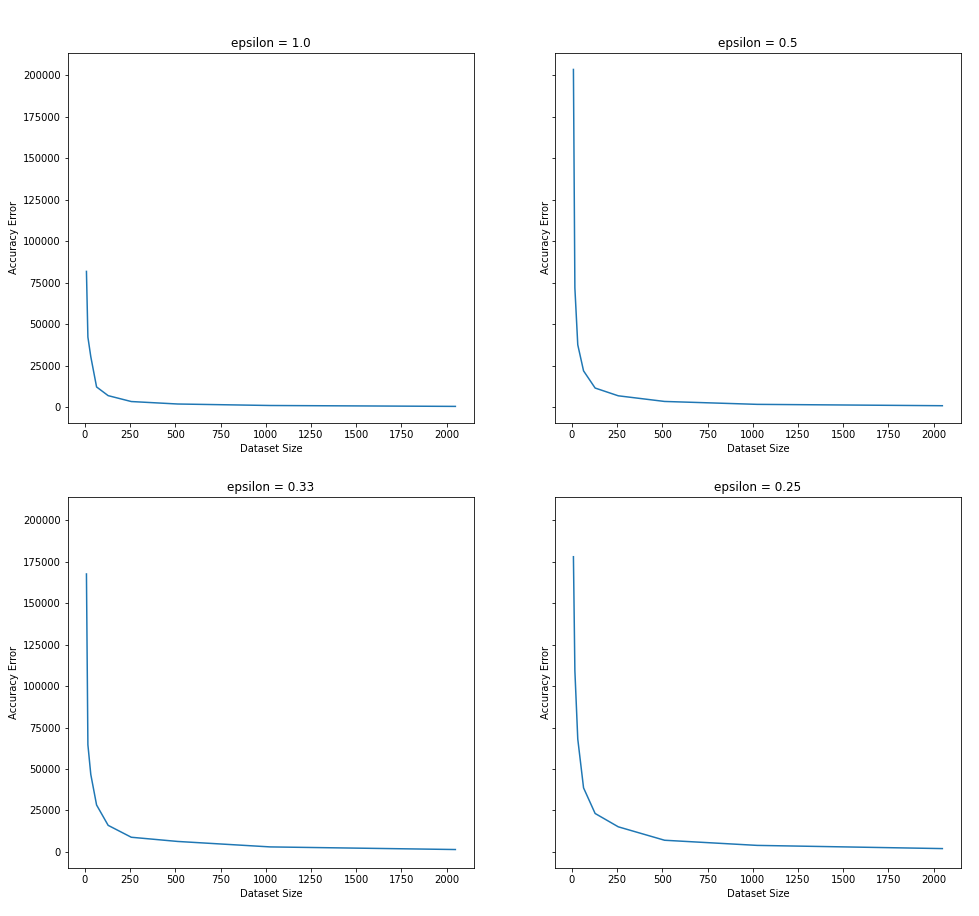
\includegraphics[width=1\textwidth]{images/increasing_ds_size.png}
    \caption{Accuracy Error for Increasing Dataset Sizes}
\end{figure}


By observing the plots, we can make a couple of conclusions:

\begin{itemize}
    \item \textbf{The smaller the epsilon gets, the bigger the accuracy error in the case of small datasets.} This, according to the definition makes sense, because small epsilon indicates higher privacy, thus for small datasets it can mean lower accuracy, due to the high amount of noise added.
    \item \textbf{The accuracy error stabilizes near 0 as the size of the dataset gets over 1000 entries.} Of course, depending to the epsilon value, this point could be earlier in the dataset sizes, as we observe for ε $= 1$. This again lays in the above mentioned property of the definition.
\end{itemize}

\subsubsection{Epsilon measurements}

The most important aspect when applying Differential Privacy to a dataset, is the selection of epsilon. This number is held accountable of the trade-off that DP offers: how much accuracy are we going to sacrifice in order to have less privacy loss, and vice versa. Given the library and our surgeries' costs dataset, we are going to measure the accuracy changes with the selection of different epsilon values.

The size of the dataset is too big, and thus the computation of the sensitivity will take too long. We assume that the data are somewhat equally distributed, thus we chose only 1\% of the dataset(which is a significant number of members), to take part in our sensitivity calculations.

In order to observe if the library functions well, we are going to compare the results produced with the \textbf{theoretical bounds of the Laplace mechanism}. 

In theory, the accuracy of an ε-differential private query, can be at most equal to the sensitivity of the query divided by epsilon, thus $$\frac{\Delta f}{\epsilon}$$ where $\Delta f$ denotes the sensitivity, and ε is our current privacy setting. 

Sensitivity is defined as the maximum difference that can be found if we alter a single entry in the dataset. We can define 2 types of sensitivity:

\begin{itemize}
    \item \textbf{Local Sensitivity} which in theory is $ \Delta f = \max_{||x-y||_1 = 1} ||f(x)-f(y)||_1$
    \item \textbf{Global Sensitivity} which we are going to use in our testings, and is defined as: $ \Delta f = \frac{upper - lower}{length(DB)} $, where upper and lower are the highest and lowest values of the column we are interested in our dataset, and length is the size of the database.
\end{itemize}

In order to compute the local sensitivity, we must check the maximum difference in the query result that occurs if we remove a single person from the database. We are going to define a function to do so, so we can check the theoretical bounds during our tests.

The results of those testings are shown in the \textbf{Figure 3.2}.

\begin{figure}[!htb]\centering
    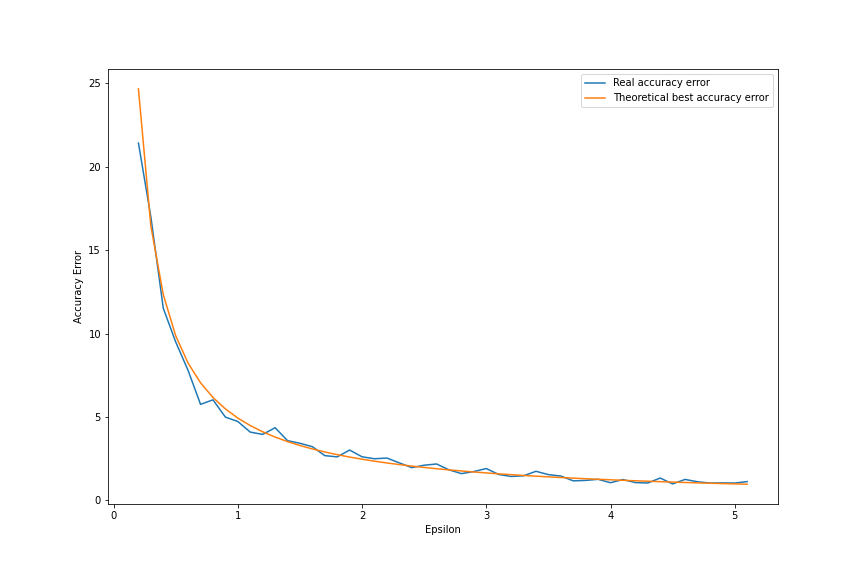
\includegraphics[width=1\textwidth]{images/epsilon_measurements.png}
    \caption{Accuracy Error for Increasing Dataset Sizes}
\end{figure}

It is clear that as we increase the epsilon value, the privacy loss gets bigger. On the other hand, if epsilon is too small, as we can see in the above plot, we are going to have extreme errors in accuracy in our queries. 

The optimal value of epsilon varies, there is no general rule for the perfect epsilon. It depends on many different aspects, such as:

\begin{itemize}
    \item The noise generated by the probabilistic mechanism used
    \item The implementation of the algorithm
    \item The size of the dataset
    \item The query itself.
\end{itemize}

Moreover, the selection of epsilon depends on the dataset. For example, we might have a dataset that is extremely important to have minimal privacy loss. In that case, we will opt to use a rather small epsilon, thus we do not disclose the sensitive data included. An other dataset could be less sensitive, but the analyst might have a need for extreme accuracy every time, so the epsilon selected should be rather big.

Regarding the comparison with the Laplace bounds, we can see that the library's query performs significantly good throughout the different epsilon values selected. This is due to the fact that IBM uses the same formula to compute the sensitivity, as well as a similar mechanism (Laplace truncated noise), in order to answer to our queries.

\subsection{Histogram Queries}

Histogram graphs are a very handy way to visualize numerical data, compare different values of a specific field, and thus extract conclusions about the dataset. We are going to study the `diffprivlib`'s method of creating an histogram, and its accuracy when changing the epsilon factor.

The IBM DP library offers a differential private way to create histograms. The difference with the simple queries that we tested, is that now, \textbf{geometric truncated} noise is added in order to satisfy DP.

\subsubsection{Metrics Used}
The result of a histogram query on a dataset is a vector containing how many entries belong on a specific range. Thus, the comparison between 2 histograms can be held out by comparing those vectors. 

There are plenty of metrics used to compare vectors, but we are going to focus on the \textbf{Euclidean Metric} and the \textbf{Kantorovich metric}(also known as Wasserstein or EMD metric). 

The euclidean metric is one of the most simple metrics, as it takes into account the distance between each pair of the 2 vectors. Thus, the distance of the vectors is defined by:

\begin{align*}
    d = \sqrt{\sum_{i=1}^n (x_i - y_i) ^ 2}
\end{align*}

where $n$ are the total elements of the vectors (must be of equal size), and $x$ and $y$ are the 2 vectors that we are comparing.

The Kantorovich metric is a more complex one, as it examines the cost to move a specific quantity of the one vector to the other, in order for the two to be similar, and thus figuring out their distance. For example, the Kant. Distance is larger if we have the vectors $[0 0 0 1]$ and $[1 0 0 0]$ than having the vectors $[0 0 0 1]$ and $[0 0 1 0]$, as in the first case the one element of the histogram is moved 3 places in order to be similar to the second one. In order to determine the cost, a base metric is used, which in our case will be the euclidean.

The way that the metric works in a naive approach, is explained in the \textbf{Figure 3.3.}

\begin{figure}[!htb]\centering
    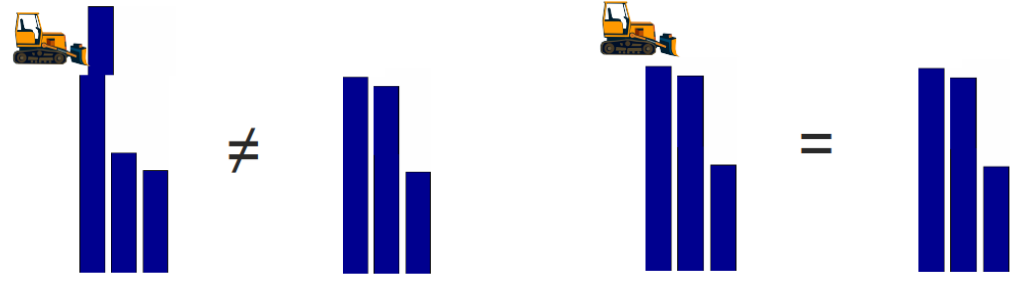
\includegraphics[width=0.7\textwidth]{images/emd.png}
    \caption{Kantorovich Metric Application on 2 histograms}
\end{figure}

This metric is much more suitable for D.P. as we are not just interested in the alteration of the results, but on the amount of alteration. If for example we are examining a histogram that contains the age of a hospital's patients, it is not the same for the private histogram to deem a 10 year old patient as 90 year old, than deeming him as 11. 

In order for the Kantorovich metric to be computed, we must solve a Dynamic Programming Problem, and make complex calculations, which are beyond of the subject of this thesis. There are many implementations of the metric, and since IBM's library is written in Python, we are going to use the QIF library %TODO:Insert mention.
which is also available as a Python library. 


\subsubsection{Bounds Definition}

In this testings we are examining salaries, thus we must set the lower and the higher bounds such as to support the most extreme salaries that could possibly be present in the dataset. Thus, the lower bound will be 0 dollars, and the higher 500,000 dollars.

\subsubsection{The identity of the testing Dataset}

During our histogram testings, we are going to use a different dataset, which contains  sensitive data regarding employee's salaries in the state of Baltimore, while stating other facts about the members of the dataset. 

The columns contained are: 
\begin{itemize}
    \item Name
    \item Job Title
    \item Annual earnings
    \item Gross earnings
\end{itemize}

We are going to focus on the last 2 columns, containing the employees' salaries. The dataset has 13000 entries, which are more than enough in order for our histograms to be realistic and accurate. The above table gives us an image of the containers of the dataset.

\begin{table}[!htb]
    \centering

    \caption{"Baltimore State Employees Salaries" dataset columns}
    \label{numbers}

    \begin{tabular}{| c | c | c | c |}
      \hline 
      Name & Job Title & Annual Earnings & Gross \\
      \hline
      Aaron,Kareem D & Utilities Inst Repair I	 & 32470.0 & 25743.94 \\
      \hline
      Abadir,Adam O	 & Police Officer &  60200.0 & 57806.13  \\
      \hline
      Abbeduto,Mack & Council Technician & 53640.0 &  59361.55 \\
      \hline
    \end{tabular}
\end{table}

\subsubsection{Simple queries}

At first, we are going to run simple instances of histogram queries, in order to take a look at the amount of error that we expect moving forward, and also familiarize with the execution of the commands. In order to create a private histogram using the library, we must provide the bins. Those should be identical to our bounds, that we have earlier defined. While creating the non-private histograms we are going to use the same bounds, in order for our comparisons to make sense. The creation of the bins and the private histogram are achieved using the following Python instructions:

\bigskip
\begin{lstlisting}[basicstyle= \footnotesize,
language=Python]
bins = np.linspace(0, 300000, 20)[1:]
result = dp.tools.histogram(input_list, bins = bins, 
         epsilon = epsilon, range=bounds_range)[0]
\end{lstlisting}
\bigskip

where epsilon is the float number selected as the epsilon parameters, and bounds range is the tuple of our dataset bounds.

The result of the execution of both the private and the non-private histogram queries for the annual earnings column are shown below, in the \textbf{Figure 3.4}.

\begin{figure}[!htb]\centering
    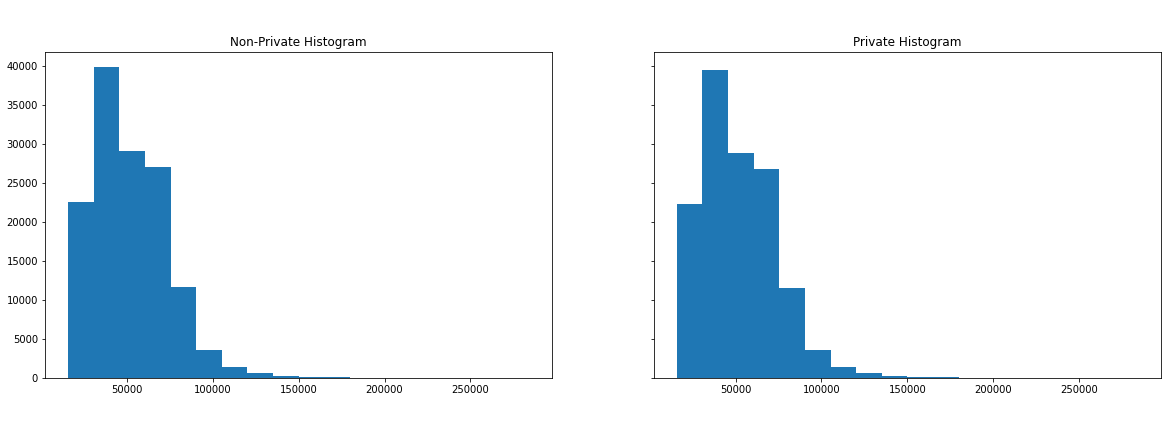
\includegraphics[width=1\textwidth]{images/simple_hists.png}
    \caption{Private and Non-private histograms for the Salaries Dataset}
\end{figure}

The results are more than satisfying in the naked eye. This is probably due to the large dataset size: we are not able to locate small changes. In order to do so, we are going to check our error using the accuracy error function that we have defined.

While applying our metrics, the Euclidean error is $14.81$, and the Kantorovich error is $91.63$. The euclidean distance error determines how many entries were wrongly classified in a bin (in average), when the differentially private query was run. So, less than 20 people out of 13.000 were wrongly classified, whereas their privacy was secured. This is quite a good trade-off!

\subsubsection{Epsilon Measurements}

Once again, we are going to run the histogram queries for different values of epsilon, in order to check their behavior as the parameter increases. The results of the execution for the Euclidean metric are shown in the \textbf{Figure 3.4}, and for the Kantorovich metric in the \textbf{Figure 3.5}. 


\begin{figure}[!htb]\centering
    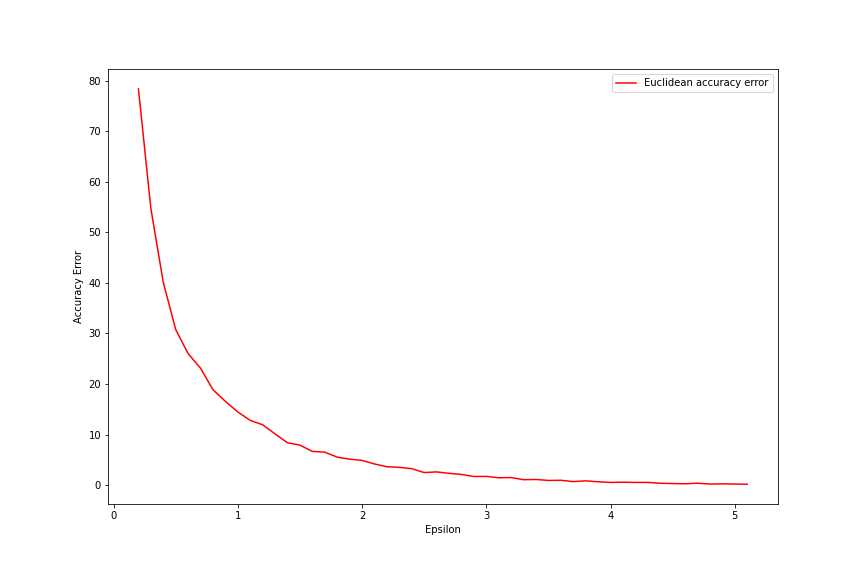
\includegraphics[width=1\textwidth]{images/hist_metrics_euclidean.png}
    \caption{Euclidean Metric Error for increasing values of epsilon}
\end{figure}

\begin{figure}[!htb]\centering
    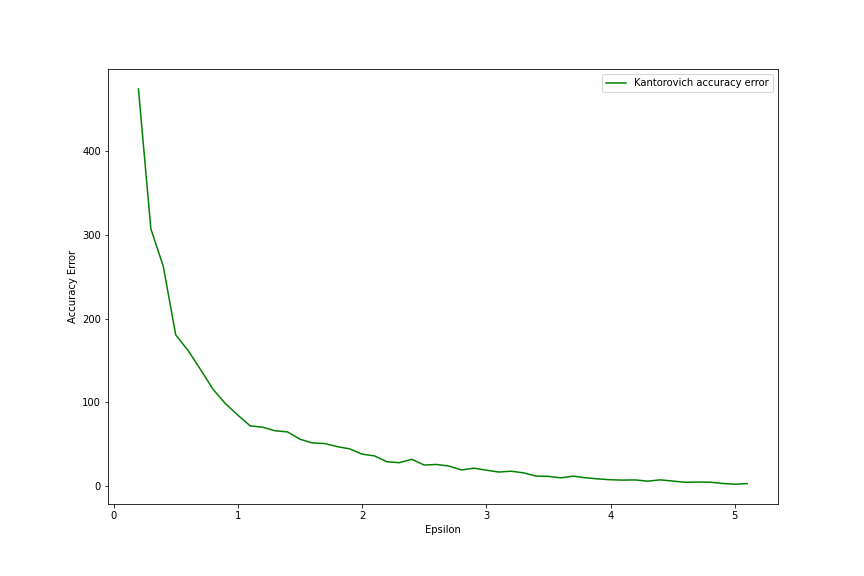
\includegraphics[width=1\textwidth]{images/hist_metrics_kantorovich.png}
    \caption{Kantorovich Metric Error for increasing values of epsilon}
\end{figure}

We observe that the error curves follow the same ratio as the previous ones, indicating what we already know, that the error decreases as the epsilon values increase. This is another case where the library produces accurate and definition-aware results. 

\subsubsection{Histogram queries in theory}
Based on [1] the histogram queries are very high sensitivity queries, thus a slight change to the bounds could be critical for their result. 

The writers suggest that we use noise generated by the LaPlace mechanism, but with a slight change. In detail they suggest the following:

\textit{"In the special (but common) case in which the queries are structurally disjoint we can do much better — we do not necessarily have to let the noise scale with the number of queries. An example is the histogram query. In this type of query the universe $N^X$ is partitioned into cells, and the query asks how many database elements lie in each of the cells. Because the cells are disjoint, the addition or removal of a single database element can affect the count in exactly one cell, and the difference to that cell is bounded by 1, so histogram queries have sensitivity 1 and can be answered by adding independent draws from $Lap(\frac{1}{\epsilon})$ to the true count in each cell."}


\subsection{Conclusions}

After a rather satisfying amount of testing in a large, real world dataset, we can safely say, that the IBM DP library has quite impressive results when it comes down to the trade-off between privacy and accuracy during both simple counting queries and histogram ones. However, we are cautious about 2 problems that we observed while using the library:

\begin{itemize}
 \item \textbf{Bounds checking}. The user must define himself the bounds, a fact that causes for speculations on the variance of the values in the dataset. It would be convenient to take the lowest and highest value in the field that we are examining, in fact that is how IBM demonstrates those examples, but that violates the rule that prevents the user from having any info of the dataset before the DP processing.
 
 \item \textbf{Non-DP preprocessing}. If we ask complicated queries (ex Surgeries performed in Stanford), the library does not offer a way to preprocess the data, thus we trust python in doing so, which results in a non-DP way of shrinking the dataset. The result that is given is of course differential private, but what happens if the dataset has only 1 record in it? That, while being a very extreme case, violates the definition of differential privacy.
\end{itemize}

The bounds' problem can be solved by running a minimum and maximum value differentially private query, which might in some cases leave some of the datasets out, but is a rather satisfying solution. 

The Non-DP preprossessing is a more tricky one, that needs special techniques in order to cover the edge case mentioned. However, we are going to check such techniques in the following section, which is based on returning the whole dataset after the application of D.P.